\section{Resultados e Discussão}
\label{sec:resultados}

Esta seção consolida as métricas obtidas nos testes de carga (k6) e no ensaio assíncrono com Cloud Tasks. As análises seguem os SLIs definidos na metodologia: latência P95, taxa de erro e comportamento das filas sob acúmulo de tarefas. O objetivo é verificar a aderência da arquitetura aos SLOs estabelecidos e compreender os pontos de saturação observados.

\begin{table}[ht]
    \centering
    \caption{Resumo dos cenários de carga e conformidade com os SLOs}
    \label{tab:resultados_k6}
    \begin{tabular}{lcccc}
        \toprule
        Cenário & Latência P95 & Throughput médio & Throughput pico & Taxa de erro \\
        \midrule
        Leitura intensiva & 158~ms & 470 req/s & 970 req/s & 0{,}00\% \\
        Mistura leitura/escrita & 658~ms & 226 req/s & 450 req/s & 0{,}00\% \\
        \bottomrule
    \end{tabular}
\end{table}

Os valores de \textit{throughput} foram extraídos diretamente dos dashboards do Cloud Run, refletindo o número real de requisições por segundo atendidas por todas as instâncias durante cada estágio do teste. Assim, VUs e req/s representam perspectivas complementares do mesmo nível de pressão sobre o sistema.

\subsection{Cenário de Leitura Intensiva}

O cenário de leitura mobilizou 1.000 usuários virtuais por 17 minutos, sustentando em média 470 requisições por segundo e alcançando um pico próximo a 970 req/s no trecho final ($900\rightarrow 1.000$ VUs). A latência P95 permaneceu em 158~ms (Tabela~\ref{tab:resultados_k6}), substancialmente abaixo do SLO de 300~ms, e nenhuma requisição apresentou erro. Esses resultados confirmam que o caminho otimizado de leitura, CDN, API em Cloud Run, Redis como cache e consultas eficientes no PostgreSQL, suporta picos significativos de tráfego sem degradação perceptível.

O Cloud Monitoring registrou o escalonamento completo das 10 instâncias de Cloud Run, atingindo CPU média de 72\% e uso de memória em torno de 31\%. Ou seja, a cota máxima de CPU foi totalmente utilizada, mas sem sinais de exaustão ou sobrecarga que pudessem comprometer as latências observadas.

\begin{figure}[ht]
    \centering
    \includegraphics[width=0.95\linewidth]{figures/fig-read-pxx.png}
    \caption{Latências P50/P95/P99 por carga (VUs) no cenário de leitura. A linha tracejada indica o SLO de 300~ms, não violado durante o teste.}
    \label{fig:latencia-leitura}
\end{figure}

\subsection{Cenário Misto (Leitura/Escrita)}

O cenário misto utilizou provisionamento automático de contas e tokens por VU, eliminando o gargalo artificial presente em versões anteriores do teste.
Com 650 usuários alternando entre 65\% de leituras e 35\% de escritas durante 21 minutos, o sistema sustentou 226 requisições por segundo ($\approx 283$ mil iterações) sem erros e manteve o SLO de 300~ms até aproximadamente 450 RPS.
A violação sistemática do SLO ocorre por volta de 539 VUs, ponto a partir do qual o Cloud Run volta a atingir o limite de 10 instâncias.

Nos estágios acima de 550 VUs, o P95 consolidado do ensaio alcançou 658~ms, enquanto o p99 atingiu 2,67~s. A origem da degradação é clara: o caminho de escrita demanda mais CPU por requisição (validações, transações ACID e invalidação de cache), reduzindo a capacidade de requisições por instância quando o limite de contêineres é atingido. As métricas do Cloud SQL mostraram estabilidade, indicando que o banco relacional não foi o gargalo primário nesse experimento.

\begin{figure}[ht]
    \centering
    \includegraphics[width=0.95\linewidth]{figures/fig-mixed-pxx.png}
    \caption{Latências P50/P95/P99 por carga (VUs) no cenário misto. A faixa tracejada marca o SLO de 300~ms; etapas acima de 539~VUs apresentam violações persistentes.}
    \label{fig:latencia-mix}
\end{figure}

A Figura~\ref{fig:comparacao} ilustra o distanciamento entre os comportamentos das duas cargas. Enquanto o cenário de leitura mantém o P95 abaixo de 200~ms mesmo no pico de 1.000 VUs, o cenário misto diverge abruptamente após 500 VUs. Esse comportamento é consistente com modelos teóricos de sistemas transacionais \cite{kleppmann_ddia_2017}, segundo os quais rotas de escrita têm custo marginal crescente e menor paralelização efetiva, sobretudo em sistemas baseados em contêineres com cotas rígidas de CPU.

\begin{figure}[ht]
    \centering
    \includegraphics[width=0.95\linewidth]{figures/fig-compare-read-vs-mixed.png}
    \caption{Comparação entre os P95 dos cenários de leitura e misto. A leitura permanece estável; a escrita viola o SLO acima de 539~VUs.}
    \label{fig:comparacao}
\end{figure}

Os resultados reforçam que, antes de adotar mecanismos mais complexos (particionamento, réplicas dedicadas ou CQRS físico), a arquitetura pode obter ganhos expressivos liberando o limite de instâncias HTTP no Cloud Run ou reduzindo o custo computacional por escrita.

\subsection{Processamento Assíncrono com Cloud Tasks}

O ensaio assíncrono publicou 51{,}58 mil tarefas em lote e monitorou a drenagem entre 01:08 e 01:18 ($\approx 10$ minutos). Isso corresponde a aproximadamente 86 tarefas/segundo processadas em média, com variação alinhada ao número de instâncias de worker ativadas dinamicamente. O Cloud Run escalou horizontalmente enquanto havia backlog, reduzindo o número de instâncias assim que o volume de tarefas diminuiu.

Nenhuma entrega foi perdida ou duplicada. A latência ponta-a-ponta permaneceu estável porque:

\begin{itemize}
    \item o Cloud Tasks opera em modo \textit{push}, eliminando \textit{polling};
    \item o Redis atuou somente como \textit{backplane} de eventos e não participou do pipeline crítico;
    \item cada worker pôde operar de forma idempotente e independente.
\end{itemize}

Esse comportamento demonstra elasticidade eficiente: a infraestrutura permanece mínima em períodos ociosos e escala agressivamente apenas durante janelas de pico, alinhando custo e demanda sem intervenção manual.

\begin{figure}[ht]
    \centering
    \includegraphics[width=0.95\linewidth]{figures/fig-queue-drain.png}
    \caption{Taxa de processamento das filas (tarefas/min) e janela de drenagem entre 01:08 e 01:18 no ensaio com Cloud Tasks.}
    \label{fig:filas}
\end{figure}

\subsection{Síntese e Discussão Integrada}

Os resultados demonstram que:

\begin{itemize}
    \item \textbf{O caminho de leitura é altamente escalável}, atendendo 1.000 VUs com folga e sem violar SLOs.
    \item \textbf{O caminho de escrita é limitado pela cota de CPU do Cloud Run}, não pelo banco.
    \item \textbf{O pipeline assíncrono é elástico e confiável}, drenando grandes volumes sem perda de tarefas.
    \item \textbf{A arquitetura é adequada para workloads dominados por leitura}, mas exige ajustes para workloads de escrita concorrente.
\end{itemize}

Esses achados orientam recomendações para escalabilidade futura, incluindo aumento das cotas de instâncias, separação de serviços de escrita, redução do custo computacional das rotas críticas e, eventualmente, adoção de padrões arquiteturais como CQRS físico ou particionamento de dados.

\subsection{Análise de Custos Operacionais e Impacto da Elasticidade}
\label{sec:custos}

Para complementar a avaliação de desempenho, esta seção compara o custo computacional dos serviços serverless utilizados (Cloud Run) com alternativas tradicionais baseadas em máquinas virtuais (Compute Engine). Todas as referências de preço utilizam os valores \textbf{Default} da região \textbf{us-central1}, garantindo consistência nas comparações.

O ponto de partida é o custo por vCPU-second. O Cloud Run adota um modelo de cobrança proporcional ao tempo efetivo de uso da CPU, enquanto o Compute Engine mantém cobrança contínua durante toda a execução da máquina virtual. Os valores considerados são:

\begin{itemize}
    \item \textbf{Cloud Run (instance-based)}: \$0.000018 por vCPU-second.
    \item \textbf{Cloud Run (request-based, ativo)}: \$0.000024 por vCPU-second.
    \item \textbf{Compute Engine C2}: \$0.033982 por vCPU-hora.
\end{itemize}

Convertendo o custo do Compute Engine para a mesma unidade utilizada pelo Cloud Run, tem-se:

\[
\frac{0.033982~\text{USD}}{3600~\text{s}} = 0.000009439~\text{USD/vCPU-second}.
\]

Com os valores normalizados, é possível calcular o fator de diferença entre os modelos:

\[
\frac{0.000018}{0.000009439} \approx 1.90,
\qquad
\frac{0.000024}{0.000009439} \approx 2.54.
\]

Assim, o Cloud Run apresenta custo unitário aproximadamente \textbf{1{,}9× (instance-based)} a \textbf{2{,}5× (request-based)} superior ao de uma vCPU otimizada do tipo C2 no Compute Engine. Essa discrepância, no entanto, não implica necessariamente maior custo operacional total.

O Compute Engine incorre em custo constante: ao provisionar uma VM, os vCPUs permanecem alocados e cobrados 24 horas por dia, independentemente da demanda. Dessa forma, workloads irregulares inevitavelmente produzem longos períodos de ociosidade, que se convertem diretamente em custo desperdiçado.

Por outro lado, o Cloud Run realiza \textit{scale-to-zero} e cobra CPU e memória apenas durante o uso efetivo. Em sistemas como o ValorizeAI, cujo tráfego é altamente variável e sensível a picos, essa característica elimina integralmente o custo ocioso. Na prática, o custo total mensal tende a ser menor, apesar do preço unitário mais alto por vCPU-second.

Uma alternativa intermediária é o Google Kubernetes Engine (GKE), que permite reduzir o custo unitário por utilizar nós Compute Engine, mas introduz novos desafios operacionais:

\begin{itemize}
    \item maior complexidade operacional (HPA, VPA, node pools, autoscaling);
    \item tempo de reação mais lento a picos repentinos;
    \item probabilidade maior de manter vCPUs ociosas em períodos irregulares.
\end{itemize}

Como resultado, o GKE costuma apresentar um custo total \textit{intermediário} entre Compute Engine e Cloud Run, porém ao custo de maior responsabilidade operacional e menor granularidade de escalonamento.

A Tabela~\ref{tab:custos_final} resume a comparação econômica, e a Figura~\ref{fig:custo-relativo} ilustra esse comportamento ao longo de um dia. Nela, o custo do Compute Engine é a linha de base (1,0); o GKE é intermediário ($\approx$1,2x); e o Cloud Run, embora atinja picos mais altos ($\approx$1,9x a $\approx$2,5x), zera o custo na ociosidade, tornando-se mais econômico para workloads variáveis.

Em síntese, mesmo possuindo custo unitário superior, o Cloud Run tende a apresentar custo operacional real menor para cargas irregulares ou sujeitas a picos abruptos, cenário típico de aplicações transacionais modernas. Já Compute Engine e GKE oferecem menor custo por vCPU-second, porém à custa de maior ociosidade ou maior complexidade operacional.

\begin{table}[ht]
\centering
\caption{Comparação econômica entre Cloud Run, GKE e Compute Engine (valores Default, us-central1).}
\label{tab:custos_final}
\begin{tabular}{lccc}
\toprule
\textbf{Serviço} & \textbf{CPU (USD/vCPU-s)} & \textbf{Elasticidade} & \textbf{Ociosidade esperada} \\
\midrule
Cloud Run (request-based) & 0.000024 & Alta & Muito baixa \\
Cloud Run (instance-based) & 0.000018 & Alta & Baixa \\
Compute Engine (C2) & 0.00000944 & Nenhuma & Alta \\
GKE (nós C2) & 0.00000944 & Moderada & Moderada \\
\bottomrule
\end{tabular}
\end{table}

\begin{figure}[ht]
\centering
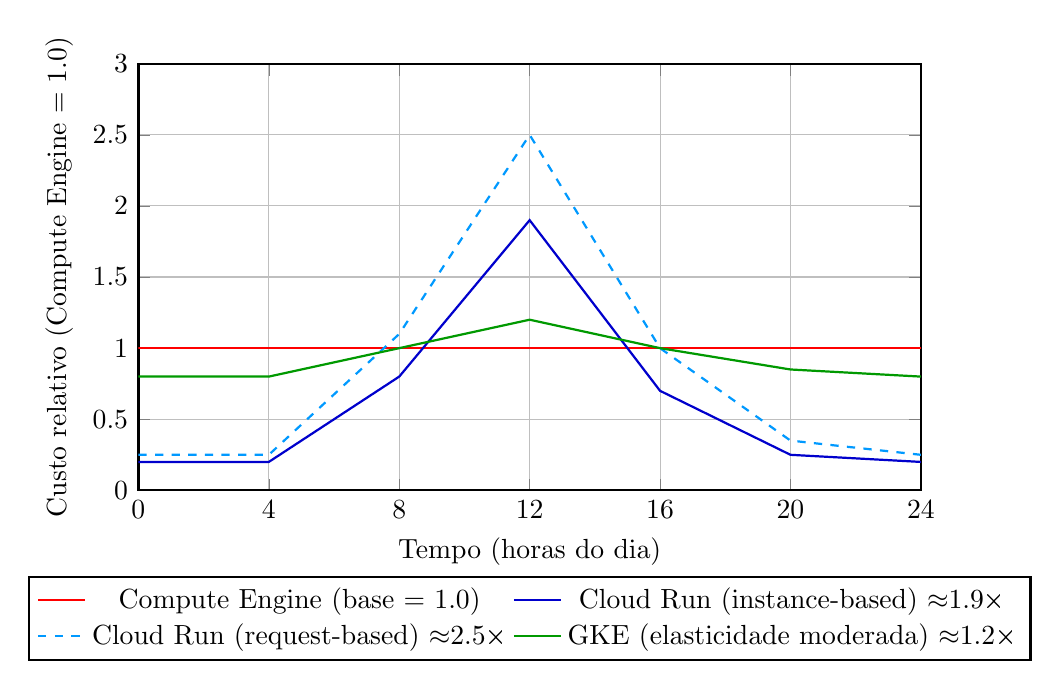
\begin{tikzpicture}
\begin{axis}[
    width=0.95\linewidth,
    height=7cm,
    xlabel={Tempo (horas do dia)},
    ylabel={Custo relativo (Compute Engine = 1.0)},
    xmin=0, xmax=24,
    ymin=0, ymax=3.0,
    xtick={0,4,8,12,16,20,24},
    ytick={0,0.5,1,1.5,2,2.5,3},
    grid=major,
    legend style={at={(0.5,-0.20)},anchor=north,legend columns=2},
    thick,
]

% Compute Engine (base = 1.0)
\addplot[red, thick] coordinates {
    (0,1.0) (4,1.0) (8,1.0) (12,1.0) (16,1.0) (20,1.0) (24,1.0)
};
\addlegendentry{Compute Engine (base = 1.0)}

% Cloud Run (instance-based) 1.9×
\addplot[blue!80!black, thick] coordinates {
    (0,0.2) (4,0.2) (8,0.8) (12,1.9) (16,0.7) (20,0.25) (24,0.2)
};
\addlegendentry{Cloud Run (instance-based) $\approx$1.9×}

% Cloud Run (request-based) 2.5×
\addplot[blue!40!cyan, thick, dashed] coordinates {
    (0,0.25) (4,0.25) (8,1.1) (12,2.5) (16,1.0) (20,0.35) (24,0.25)
};
\addlegendentry{Cloud Run (request-based) $\approx$2.5×}

% GKE (~1.2×)
\addplot[green!60!black, thick] coordinates {
    (0,0.8) (4,0.8) (8,1.0) (12,1.2) (16,1.0) (20,0.85) (24,0.8)
};
\addlegendentry{GKE (elasticidade moderada) $\approx$1.2×}

\end{axis}
\end{tikzpicture}
\caption{Custo relativo entre Compute Engine, Cloud Run e GKE, normalizado para Compute Engine = 1.0.}
\label{fig:custo-relativo}
\end{figure}
